% ------------------------------------------------------------------------------
% Este fichero es parte de la plantilla LaTeX para la realización de Proyectos
% Final de Grado, protegido bajo los términos de la licencia GFDL.
% Para más información, la licencia completa viene incluida en el
% fichero fdl-1.3.tex

% Copyright (C) 2012 SPI-FM. Universidad de Cádiz
% ------------------------------------------------------------------------------

Este capítulo trata sobre todos los aspectos relacionados con la implementación del sistema en código, haciendo uso de un determinado entorno tecnológico.

\section{Entorno de Construcción}
%En esta sección se debe indicar el marco tecnológico utilizado para la construcción del sistema: entorno de desarrollo (IDE), lenguaje de programación, herramientas de ayuda a la construcción y despliegue, control de versiones, repositorio de componentes, integración contínua, etc.

El framework empleado en la creación de esta página web es \textit{\textbf{Grails}}, un framework para aplicaciones web libre desarrollado sobre el lenguaje de programación \textit{\textbf{Groovy}} (el cual a su vez se basa en \textit{\textbf{Java}}). Groovy posee una sintaxis muy parecida a \textit{Java}, comparte el mismo modelo de objetos, de hilos y de seguridad, además, puede acceder directamente a todas las API existentes en \textit{Java}. Esta relación entre ambos lenguajes, ha permitido que algunas partes del desarrollo se haya empleado \textit{Java} y en otras \textit{Groovy}.\\

Para emplear estos lenguajes en el desarrollo, se emplea el IDE \textit{\textbf{Grails Tool Suite}}, un entorno de trabajo donde podemos aplicar el paradigma \textbf{Modelo Vista Controlador} (MVC).\\

\textit{Grails Tool Suite} es un IDE altamente productivo que sigue paradigmas como convención sobre configuración o no te repitas (DRY) proporcionando un entorno de desarrollo estandarizado y ocultando gran parte de los detalles de configuración al programador.\\

Una de las ventajas que proporciona este tipo de proyectos, es que podemos instalar dependencias y \textit{plugins} que nos permitan instalar utilidades a nuestro proyecto Grails para ser empleadas directamente sobre el código y aplicar el paradigma DRY que se ha explicado anteriormente. Algunos de ellos son:

\begin{itemize}
	\item \textit{tomcat} Para instalar el contenedor de Java Tomcat.
	\item \textit{jquery} Para instalar JQuery en el proyecto.
	\item \textit{spring-security-core} Para realizar la securización de la aplicación web.
	\item \textit{executor} Para realizar tareas en segundo plano.
	\item \textit{apache.poi} Para la creación de documentos word, excel o pdf.
	\item \textit{mysql-connector-java} Para permitir la conexión de la aplicación con MySQL.
\end{itemize}

Todo el código de la aplicación se encuentra ubicado en un espacio de trabajo de Assembla cuya dirección es \url{https://app.assembla.com/spaces/systematic-literature-review/} que puede ser descargado en un equipo por Subversion (SVN). En este espacio de trabajo se ha insertado además todo el contenido de la memoria así como recursos necesarios que puedan ser de utilidad para este trabajo.

\section{Código Fuente}
%Organización del código fuente, describiendo la utilidad de los diferentes ficheros y su distribución en paquetes o directorios. Asimismo, se incluirá algún extracto significativo de código fuente que sea de interés para ilustrar algún algoritmo o funcionalidad específica del sistema.

En la figura \ref{fig:estruc-grails} podemos ver la estructura de directorios que tiene este proyecto Grails.\\

\begin{figure}[!hpt]
	\begin{center} 
		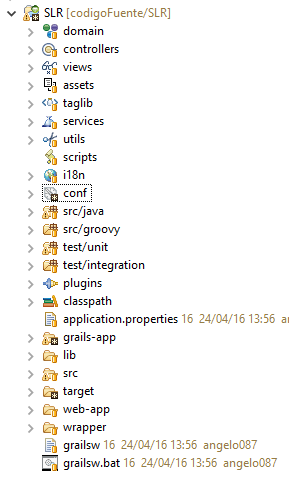
\includegraphics[scale=0.6]{estructura-grails-project.png}
		\caption{Estructura Proyecto Grails}
		\label{fig:estruc-grails}
	\end{center}
\end{figure}

\begin{itemize}
	\item \textbf{conf} Archivos de configuracion
	\item \textbf{controllers} Controladores
	\item \textbf{domain} Entidades
	\item \textbf{i18n} messages bundles
	\item \textbf{services} Servicios
	\item \textbf{taglib} Libreria de etiquetas
	\item \textbf{util} Clases de utilidad
	\item \textbf{views} Vistas
	\item \textbf{layouts} Layouts SiteMesh
	\item \textbf{lib}
	\item \textbf{scripts}
	\item \textbf{src}
	
	\begin{itemize}
		\item \textbf{groovy} Otras clases Groovy
		\item \textbf{java} Otras clases Java
	\end{itemize}
	
	\item \textbf{test} Casos de prueba
	\item \textbf{web-app} Raiz de la aplicacion web
\end{itemize}

\section{Scripts de Base de datos}
Organización del código fuente, describiendo la utilidad de los diferentes ficheros y su distribución en paquetes o directorios. Asimismo, se incluirá el script de algún disparador o un procedimiento almacenado, que sea de interés para ilustrar algún aspecto concreto de la gestión de la base de datos.
